%%=============================================================================
%% Onderzoek
%%=============================================================================

\chapter{Onderzoek}
\label{ch:onderzoek}

In dit hoofdstuk wordt dieper ingegaan op de verschillende caching -en synchronisatie methodes, hun toepassing op de businesscase en het proces voor het implementeren van synchronisatie. Volgende onderdelen komen aan bod in dit hoofdstuk:
\begin{itemize}
\item Online/Offline status registstratie
\item Caching, preloading en Read-Only Optimised
\item Planning bij het bepalen van synchronisatie
\item Last/First Write Wins en Conflict resolution
\item De gebruikte AWS services voor de synchronisatie in de backend
\end{itemize}

\section{Online/Offline status registratie}
Voor dat de verschillende caching- en synchronisatie methodes kunnen worden overlopen, is het belangrijk om te onderzoeken hoe de applicatie op een betrouwbare manier de status van de internetverbinding kan controleren. De status van de verbinding vormt immers de belangrijkste voorwaarde bij de beslissing om de data\footnote{de request, in het geval van de business case}  al dan niet te cachen.
\clearpage
\begin{enumerate}
\item DOM API's aanspreken vanuit JavaScript. Helaas is er geen consistente\autocite{offline-spec-mozilla} cross-browser support op het controleren van de status van de verbinding zonder gebruik te maken van van requests naar externe data. Een voorbeeld is luisteren naar events van het document.window object om online en offline status te controleren werkt niet op alle browsers. Een andere optie waarbij de status van de verbinding wordt opgevraagd met window.navigator.onLine werkt ook niet consistent in alle browsers.
\item Een request uitvoeren naar een externe bron: als de applicatie een request uitvoert naar een externe bron en de HTTP code controleert van de respons, dan kan de applicatie gemakkelijk afleiden wat de status van de verbinding is. Deze methode garandeert dat de applicatie correct kan vaststellen wanneer de status van de verbinding verandert. Deze methode ook gebruikt in libraries zoals Offline.js\footnote{Zie https://github.com/hubspot/offline}.
\end{enumerate}

\begin{lstlisting}[caption=Verschillende methodes\autocite{offline-online-examples} voor controleren offline en online status.]
    // met jQuery
    $(window).bind("online", applicationBackOnline); 
    $(window).bind("offline", applicationOffline);

    //IE met vendor specifieke objecten
    window.onload = function() {
        document.body.ononline = ConnectionEvent;
        document.body.onoffline = ConnectionEvent;
    }
    // Met gebruik van event listeners
    document.body.addEventListener("offline", function () {
    //alert("offline")
    }, false);
    document.body.addEventListener("online", function () {
    //alert("online")
    }, false);
    
    // met native window.navigator
    if (navigator.onLine) {
  	// Online
     } else {
  	// Offline
	}
    
\end{lstlisting}
\clearpage
\section{Caching van requests}
Voor het onderzoek werd geopteerd op gebruik te maken van de methode waarbij een call wordt uitgevoerd om te controleren of de client online of offline is. Wanneer de applicatie registreert dat er geen verbinding meer is, worden alle POST/PUT/UPDATE\footnote{Alle requests die geen POST/PUT/UPDATE request zijn worden genegeerd want die hebben geen invloed op de synchronisatie} requests gecached als afzonderlijke objecten in localStorage. Hiervoor wordt er gebruik gemaakt van localForage. Wanneer de applicatie terug online is, wordt er 1 request naar de server alle gecachte data doorgestuurd. Requests die een UPDATE uitvoeren op een object dat aangemaakt werd (CREATE) tijdens de offline status, worden allemaal gebundeld in een enkel object. Op die manier wordt de volgorde gegarandeerd voor het verwerken van de verschillende requests. Wanneer er dan synchronisatieproblemen optreden, moeten die in de lambda's worden opgevangen die de individuele request moeten verwerken.

\begin{lstlisting}[caption=Caching van een request]
private cache(key: string, command: Request) {
	// Haalt de huidige cache uit localStorage als Promise
	return storage.getItem<Action[]>(key).then(actions => {
		// Default lege array indien actions niet bestaat
		actions = actions || [];
	
		// Omzetten van request naar data object
		const data: any = command.serialize();
		data.method = command.method;
		data.path = command.path;
		
		// Toevoegen aan array van requestobjecten
		actions.push(data);
		
		// Terug in storage plaatsen wanneer gecachte actie is toegevoegd
		// localForage blibliotheek kiest opslagmedia (localStorage of IndexedDB)
		return storage.setItem<Action[]>(key, actions);
	});
}
\end{lstlisting}

De connectie status van de de applicatie wordt bewaard als state in de redux store. Die kan worden opgevraagd als een Observable wanneer requests moeten worden uitgevoerd naar de backend of voor het tonen van een waarschuwing in de UI. Wanneer de status van de verbinding zou wijzingen, dan wordt de subscribe methode opnieuw aangeroepen. Op die manier kunnen verschillende configuraties worden ingesteld afhankelijk van de verbinding.

\begin{lstlisting}[caption=Opvragen van de status van de verbinding aan de hand van de redux store]
	// Bevragen van de store
	this.store.select(state => state.common.network.online)
		// Retourneert een Observable
		.subscribe( online => 
		// reactie op boolean 'online'
	)
\end{lstlisting}
		
\begin{figure}[h]
\caption{Caching van requests in de client}
\centering
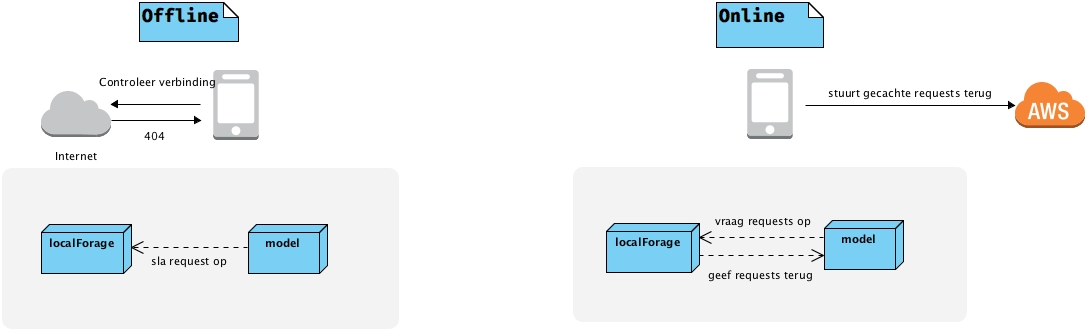
\includegraphics[width=1\textwidth]{caching-requests}
\end{figure}

\section{Data preloading in de client}
Bij een applicatie die zowel online als offline moet werken, is het belangrijk dat de data wordt preloaded\footnote{Preloading is het op voorhand inladen van data.} in de applicatie. Zo kan de gebruiker blijven verder werken indien de applicatie plots offline is. De redux store is de SSOT en bevat de preloaded data in-memory. De applicatie kan de preloaded data uit de store gebruiken bij het laden van de views.
 Het belangrijkste aandachtspunt is hierbij de schaalbaarheid van de oplossing. In de business case van Pridiktiv worden verschillende requests naar de server uitgevoerd naar de server om de data op te vragen. Wanneer de functionaliteit en data capaciteit van de applicatie toeneemt kan het aantal requests kan wel dramatisch stijgen. Door het single-threaded karakter van JavaScript is het echter niet mogelijk om parallel te werken. Een mogelijke oplossing voor dat probleem kan een web worker\autocite{webworker-explained} zijn.
 
\subsection{Beperkingen door single-threaded omgeving}
JavaScript is een single-threaded omgeving waardoor meerdere scripts niet parallel kunnen worden uitgevoerd. Dit vormt problemen wanneer een webapplicatie UI events, queries, een groot volume API data en tegelijk de DOM aanpassingen moet verwerken. Met technieken zoals setTimeout() en setInterval() is het mogelijk om concurrency te simuleren maar dit maakt de applicatie meteen een stuk complexer. Dankzij de HTML5 specificatie is het mogelijk om Web Workers te gebruiken. Deze laten toe om scripts in de achtergrond uit te voeren. Hierdoor is het mogelijk om complexe berekeningen concurrent uit te voeren zonder dat dit een performantie impact op de applicatie heeft.

\subsection{Preloading methodes}
Er zijn 3 methodes voor preloading die van toepassing zijn voor de business case.

\subsubsection{Serieel inladen van de data}
Bij deze methode wordt de data serieel opgevraagd van de server. Dit is de minst complexe oplossing en is ideaal wanneer het volume van de data beperkt is. Echter, hoe groter het data volume, hoe groter de impact op de performantie van de client applicatie. Door de vele requests en de vele aanpassingen van de in-memory Redux state wordt de main thread geblocked waardoor de UI niet kan worden gerenderd. Dit wekt de indruk bij de gebruiker dat de applicatie niet responsief is. Deze methode is dus enkel geschikt wanneer er maar een beperkt aantal requests zijn.

\subsubsection{Web worker}
\label{sssec: web-worker}
Aan de hand van web workers is het mogelijk om parallel een ander Javascript applicatie te gebruiken. De API voor web workers wordt door alle \autocite{web-worker-support} moderne browsers ondersteund. Met behulp van web workers is het mogelijk om CPU-intensieve taken onafhankelijk van de web pagina uit te voeren. Als men dit toepast op preloading kunnen web workers een van de volgende taken op zich nemen.

\begin{enumerate}
\item Data ophalen van de server en verwerken naar een state object.
\item Omzetten van response/data object naar state object voor de redux store
\end{enumerate}

\begin{figure}[h]
\caption{Web worker die request verwerkt}
\centering
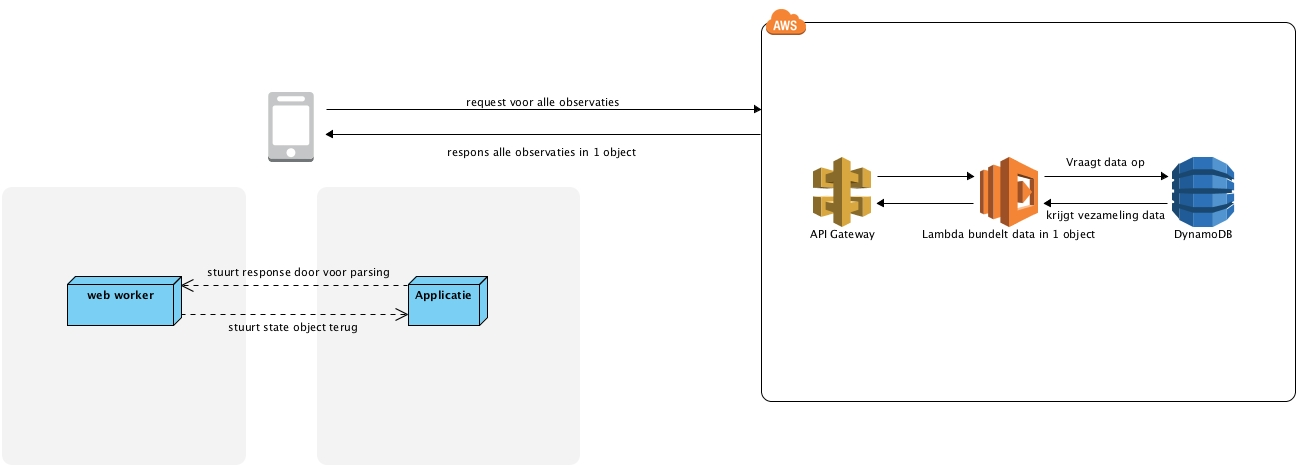
\includegraphics[width=1\textwidth]{example-webworker}
\end{figure}

Een nadeel bij web workers is de complexiteit wanneer externe scripts worden gebruikt. Als er meerdere dependencies zijn voor het uitvoeren van de code of als een superset zoals TypeScript wordt gebruikt, dan moet men gebruik maken van SystemJS\footnote{SystemJS is een dynamische module loader voor JavaScript ES6}. SystemJS is echter niet combineerbaar met Angular CLI, de build tool die gebruikt wordt bij de business case. Door deze beperking is het werken met web workers niet de ideale oplossing voor de business case. Het is ook mogelijk om de Webpack\footnote{Webpack is een module bundler. Webpack laadt net als SystemJS de verschillende modules in maar bundelt die ook netjes in verschillende files. Op die manier moet een applicatie die heel wat dependencies heeft, enkel maar een file inladen. }-configuratie file die Angular CLI gebruikt handmatig te configureren. Dit wordt echter sterk afgeraden omdat de meerwaarde van de bundling die door Angular CLI wordt uitgevoerddan volledig verloren gaat.

\begin{lstlisting}[caption=Creatie van een web worker]
TODO
\end{lstlisting}

\begin{lstlisting}[caption=Communicatie tussen applicatie en webworker]
TODO
\end{lstlisting}

\subsubsection{Redux state server side opbouwen met Read-Only Optimised}
\label{sssec: redux-server-side}
Een derde methode is het opzetten van een redux state in de backend die door de client kan worden opgevraagd. Op die manier moet enkel het state object worden toegevoegd aan de store wanneer het is opgevraagd van de server. Een nadeel van deze methode is de state van de client die nu sterk gekoppeld is aan de backend. Grote voordeel is dat de backend nu verantwoordelijk is voor alle intensieve operaties en dat de client applicatie enkel maar zijn state moet injecteren in de store. Bij deze methode kan de Read-Only Optimised techniek gebruikt worden bij het opstellen van de client state.

\subsubsection{Toepassing business case}
In de business case wordt de request serieel bevraagd van de server. Nadat de pati\"entenlijst is opgevraagd, worden voor alle pati\"enten de relevante data opgevraagd. In de piloot versie waren dat ongeveer 75 personen die elk taken, notities, observaties, medische parameters en wondzorgdossiers kunnen bevatten. Dit leidt tot een 500 requests die in een zeer korte periode worden uitgevoerd. Het gebruik van web workers \autocite{webworker-reference} gecombineerd met een gebundelde data zou het aantal requests sterk kunnen verminderen. In de business case is er ook sprake van afbeeldingen die moeten worden gesynchroniseerd met de applicatie maar het cachen van BLOBs valt buiten de scope van dit onderzoek.

\section{Data synchronisatie: planning bij development}
Wanneer een synchronisatieoplossing moet worden ontwikkeld voor een applicatie, is het belangrijk om alle use cases in kaart te brengen waarbij er rekening moet worden gehouden met synchronisatie. Dit zorgt ervoor dat er geen functionaliteit over het hoofd wordt gezien bij het ontwikkelen van de synchronisatieoplossing. Ter illustratie wordt in de onderstaande voorbeeld de business case van Pridiktiv ontleed.

\begin{center}
    \begin{tabular}{ l | r }
    \hline
    Functionaliteit & Synchronisatie \\ \hline
    Taken & First-Write Wins of conflict resolution \\
    Observaties & geen conflict mogelijk \\
    Medische data & geen conflict mogelijk \\
    Wondzorg & First-Write Wins of conflict resolution \\
    Notities & Geen conflict mogelijk \\
    \hline
    \end{tabular}
\end{center}

De onderverdeling is het uitgangspunt voor de volgende stap namelijk het bepalen van de verschillende synchronisatie mogelijkheden. Zo kan bijvoorbeeld worden bepaald dat de gebruiker bij een conflict zelf een beslissing moet nemen. Of indien er een conflict optreedt bij een synchronisatie van bepaalde data, dat er automatisch voor Last/First Write Wins wordt gekozen. In het geval waarbij er conflict resolution moet gebeuren door de gebruiker, kunnen kan worden bepaald welke keuzes de gebruiker krijgen en welke keuzes de server zelf kan maken. Bovenstaande overzicht vormt dan als het ware de basis voor de ontwikkeling van de synchronisatie. Een ander voorbeeld is het deactiveren van bepaalde functionaliteit bij wanneer de applicatie offline is. Hierdoor kunnen potentieel complexe synchronisatieproblemen worden vermeden. Dit heeft echter als nadeel dat de applicatie niet meer de volledige functionaliteit kan aanbieden wanneer de verbinding is verbroken. Het al dan niet uitschakelen van bepaalde functionaliteit bij offline gebruik is sterk afhankelijk van de business case

\section{Read-Only Optimised}
De belangrijkste insteek voor deze methode is om zo effici\"ent mogelijk gebruik te maken van de bandbreedte van de client of processor tijd serverside. Read-Only Optimised is dan ook eerder een optimalisatietechniek dan een synchronisatiemethode. Deze techniek laat toe om enkel nieuwe data binnen te halen waardoor data die de applicatie reeds bezit niet opnieuw worden opgevraagd. De complexiteit van deze methode stijgt evenredig met het aantal parameters dat in de data kan worden aangepast. Deze methode wordt vooral gebruikt bij het cachen van data voor offline gebruik.
\subsection{Overzicht: Client}
Bij Read-Only Optimised staat de synchronisatie van de client centraal. Tijdens de periode dat de client offline was, is het mogelijk dat er nieuwe data zijn aangemaakt. Om deze data te synchroniseren kan de client alle data opnieuw opvragen maar deze manier heeft enkele nadelen. Indien de data klein is zoals enkel tekst, dan is Read-Only Optimised triviaal en kunnen alle data opnieuw worden opgevraagd. Wanneer er echter grotere data moet worden ingeladen zoals afbeeldingen, dan kan Read-Only Optimised heel wat bandbreedte uitsparen. Dankzij de ngrx store is het ook gemakkelijk om manipulaties uit te voeren op de data, waardoor er eenvoudig objecten kunnen worden toegevoegd aan de data in de store. Belangrijke voorwaarde voor het uitvoeren van deze actie is het bijhouden in de client van de timestamp van de laatste update indien de data aanwezig zijn. Indien er geen timestamp aanwezig is, dan weet de client dat alle data moeten worden opgevraagd.
\subsection{Overzicht: Server}
De server houdt rekening met de verschillende timestamps om te bepalen welke data er moet worden geretourneerd.

\subsection{Opmerkingen}
Ondanks de perceptie dat dit een eenvoudige methode is om te implementeren, zijn er enkele opmerkingen zij deze methode:
\begin{enumerate}
\item In bovenstaand scenario wordt er enkel maar uitgegaan van nieuwe data, dus CREATE operaties. Indien de methode ook voor UPDATE moet werken is het in bepaalde gevallen noodzakelijk om ook de databank structuur aan te passen.
\item Bij klassieke SQL databanken kan gemakkelijk worden gefilterd op bepaalde velden zoals een 'updated veld' binnen een tabel. Bij DynamoDB is dit moeilijker als de waarde van de query geen deel uitmaakt van de sort -of partition key. In dat geval moet er dan gebruik worden gemaakt van een extra secondary index niet telkens alle partition key moet worden overlopen telkens wanneer er een GET request is.
\item Het is bij kleine data vaak eenvoudiger om steeds alle data op te vragen en geen gebruik te maken van de Read-Only Optimised methode. De complexiteit die Read-Only Optimised toevoegt bij eenvoudige scenario's maakt deze methode soms overbodig.
\end{enumerate}
\subsection{Toepassing}
Met behulp van twee timestamps wordt er bijgehouden wanneer de laatste GET is uitgevoerd en wanneer de laatste aanpassing in een tabel heeft plaatsgevonden. Op die manier kan de backend bepalen welke informatie er moet worden geretourneerd. Wanneer er maar een beperkt volume data wordt geretourneerd dan zorgt de Read-Only Optimised methode nodeloos voor extra complexiteit. Het is daarom enkel aangeraden om enkel Read-Only Optimised te gebruiken indien er met grotere datasets wordt gewerkt.
\subsubsection{Toepassing op de business case}
In de backoffice en mobiele applicatie van Pridiktiv wordt er momenteel geen gebruikt gemaakt van Read-Only Optimised. Het Read-Only Optimised patroon zou in de business case van Pridiktiv eerder geschikt zijn wanneer de state server side wordt opgebouwd. Als de state voor de caching serverside wordt opgebouwd, dan zou men gebruik kunnen maken van Read-Only Optimised. Door de opgebouwde state te persisteren en de tegelijk  de timestamps van de laatste change binnen een bepaalde categorie bij te houden in een 'changes' tabel zou het aantal queries dat nodig is om de state op te bouwen sterk kunnen verminderen. 

\section{Last/First Write Wins}
Bij Last/First Write Wins gaat er onherroepelijk informatie verloren. Afhankelijk van de gekozen conflict resolution methode is het wordt de eerste of laatste write bijgehouden. Dit is de eenvoudigste manier van conflict resolution maar men moet bereidt zijn om een compromis te sluiten en informatie op te offeren in ruil voor minder complexiteit bij het synchroniseren. Wanneer heel snel naar een offline/online synchronisatiemethode moet worden gezocht, biedt die de gemakkelijkste oplossing.
\subsection{Overzicht: Client}
Bij deze methode is de impact van de client miniem want de client weet niet dat er een synchronisatieprobleem zal optreden wanneer die data doorstuurt naar de server.
\subsection{Overzicht: Server}
Deze methode vind plaats wanneer verschillende clients een verandering aanbrengen bij hetzelfde bestaande object. Hierdoor krijgt de databank verschillende waarden binnen en moet dat verplicht de databank er toe om te reageren. Afhankelijk van de methode die gekozen zijn er twee scenario's mogelijk bij deze synchronisatiemethode.
\begin{enumerate}
\item First Write Wins. Hier wordt enkel de eerste write van een object of row bijgehouden. Indien hetzelfde object opnieuw wordt aangepast dan wordt er een exceptie geworpen. Dit is enkel maar mogelijk in use cases waarbij een aanpassing in een object finaal is. Een voorbeeld uit de use case is bijvoorbeeld het volbrengen van een taak. Wanneer een taak is volbracht, is het niet meer mogelijk om die aan te passen. Met behulp van een completed flag kan de state van de taak worden bijgehouden. Wanneer de aanpassingen in een object niet finaal zijn, is een last Write wins een betere methode.
\item Last Write Wins. Bij Last Write Wins wordt enkel maar de laatste write operatie behouden. Er wordt geen vergelijking gemaakt met de waarde die reeds in de databank beschikbaar is en de nieuwe waarde die wordt doorgegeven. Men hanteert deze methode dan best enkel bij bestaande objecten waarbij het mogelijk is om UPDATE operaties op uit te voeren.
\end{enumerate}
\subsection{Opmerkingen}
First/Last Write wins is een aantrekkelijke methode wanneer er op korte termijn synchronisatie moet worden gerealiseerd maar er zijn wel enkele bemerkingen bij deze methode.
\begin{itemize}
\item Er gaat onherroepelijk data verloren op deze manier. Indien de use case dit niet toelaat dan moet er worden gekeken naar andere conflict resolution policy.
\item Het type van de data (finaal of niet-finaal) sluit de andere methode uit. Niet-finale data met First Write Wins maken de data impliciet finaal en immutable.
\end{itemize}
\subsection{Toepassing}
\subsubsection{Toepassing op de business case}
Momenteel hanteert de backend van Pridiktiv enkel een First/Last Write principe bij data. Naar de toekomst zou dit moeten veranderen naar een een bredere oplossing die conflict resolution kan aanbieden.

\section{TODO ergens tussenplaatsen}
De API Gateway geeft het object door aan de proxy lambda die de objecten op een queue plaatst.  Een andere lambda leest alle boodschappen uit de queue en stuurt elke request terug naar de gateway lambda. De API Gateway wijst de correcte lambda aan die verantwoordelijk is voor de verwerking van de oorspronkelijke request.

\section{Conflict Resolution}
Bij synchronisatie gaat er idealiter geen informatie verloren of laat de business case gaan dataverlies toe. Daarom is het ook belangrijk om te kijken hoe data kan worden gesynchroniseerd op een manier waarbij geen data verloren gaan. Om het onderzoek binnen de restricties van de business case te laten passen, worden hier enkel AWS services gebruikt bij het synchronisatie. Een andere belangrijke opmerking dat het enkel maar gaat over UPDATE en DELETE operaties want Een CREATE operatie kan niet leiden tot een conflict wanneer het toestel offline is.
\subsection{Overzicht: Client}
Net zoals bij First/Last Write Wins, is de rol van de client beperkt. Wanneer de data zonder timestamp in de database wordt bewaard, is het belangrijk om een timestamp bij te houden wanneer nieuwe data zijn aangemaakt of aangepast. Zo heeft de server een referentiepunt om de data te verwerken.
\subsection{Overzicht: Server}
Timestamps bieden een eenvoudige oplossing om de controleren wanneer een bepaalde actie heeft plaatsgevonden. De timestamp van het nieuwe aangepaste object wordt vergeleken met de timestamp van het object dat reeds aanwezig is in de database. Zo kan bijvoorbeeld een timestamp worden bijgehouden in een 'modified' veld. Dat veld kan worden vergeleken met de timestamp van de UPDATE of DELETE die wordt doorgestuurd. Zo kan de server bepalen of er al dan niet een conflict is en wat er in het geval van een conflict moet gebeuren. Indien er geen timestamp sinds de laatste update wordt bewaard in het object, dan wordt synchroniseren zeer moeilijk en is First/Last Write Wins een betere oplossing. Het bijhouden van een timestamp alleen is echter niet voldoende. Het is belangrijk om op voorhand te bepalen wat de conflict resolution policies zijn en welke uses cases er allemaal van toepassing zijn. Niet alle conflicten kunnen worden opgevangen door de server. Zo kan de server geen beslissing nemen wanneer een DELETE actie wordt uitgevoerd op een object en er na nog een update wordt doorgestuurd. De gebruiker moet dan een waarschuwing krijgen dat zijn object is verwijderd en dan zijn aanpassingen niet zijn opgeslagen. Indien de gebruiker geen boodschap zou krijgen, dan wekt de server de perceptie dat er iets fout is gegaan bij de verwerking van de data.
\subsection{Toepassing}
\subsubsection{Toepassing op de business case}
\subsubsection{UPDATE operatie}
Pridiktiv maakt gebruik van DynamoDB voor het bijhouden van de data. In DynamoDB wordt er gewerkt met een Partition Key die kan worden vergeleken met een Primary Key in SQL-terminologie en optioneel een Sort Key die  de Partition Key bevat in combinatie met een attribuut van het object. Daarnaast is het ook nog mogelijk om Secondary Indices te cre\"eren die functioneren zoals Sort keys.  Het is belangrijk dat de timestamp de Partition Key is of deel uitmaakt van de samengestelde Sort Key. Indien niet, is de DynamoDB verplicht om een full table scan uit te voeren op de tabel en over die data set te filteren. Omdat de timestamp deel uitmaakt van de Primary Key, is het bij updates eenvoudig om bij te houden wanneer de laatste update is uitgevoerd en om te voorkomen dat een UPDATE gedupliceerd wordt. Dit laatste wordt vermeden doordat de Partition Key unique moet zijn en dus met andere woorden kan die niet worden gedupliceerd zonder dat DynamoDB een exceptie gooit.
\subsubsection{DELETE operatie}
Het is in de business case van Pridiktiv niet mogelijk om date te verwijderen. Alle data moet zichtbaar blijven in een historiek. Hierdoor is het niet toegelaten om DELETE operaties uit voeren, enkel UPDATE operaties. 
\section{Open-source libraries}
Voor het synchroniseren van de data bij Pridiktiv in AWS wordt er gebruik gemaakt van twee verschillende Open Source libraries. Deze zijn gemaakt om een oplossing aan te bieden voor Pridiktiv en in kader van dit onderzoek. De componenten zijn geschreven in JavaScript voor NodeJS 4.3 en hoger. Hierdoor is het mogelijk om nieuwere features uit ES6 te gebruiken zoals Promises. Het is specifiek ontwikkeld om te werken met Simple Queue Service van AWS maar biedt de flexibiliteit om gebruikt te worden buiten AWS Lambda, bv in AWS EC2 instances die ook NodeJS gebruiken. Deze libraries zijn ontwikkeld in kader van dit onderzoek en worden gebruikt binnen de productieomgeving van de Pridiktiv applicaties.
\subsection{aws-sqs-push}
Deze library heeft een functie die berichten op de SQS queue plaatst en een Promise retourneert wanneer er een bericht op de queue is geplaatst. De naam van de queue wordt met een hulpfunctie aws-sqs-geturl opgevraagd. Op deze manier is de gebruiker van deze library niet verplicht om de volledige ARN naam van de SQS door te geven. Wanneer de mesage een object bevat is dan wordt het object met JSON.stringify() automatisch omgevormd naar een string.

\begin{lstlisting}[caption=Voorbeeld dat data plaatst op een SQS queue met behulp van de aws-sqs-push library]

	const sqsPush = require('aws-sqs-push');

	sqsPush('QueueName', 'SomeMessage').then(messageId => {
    		console.log(messageId);
    	//=> '8a98f4d0-078b-5176-9af2-bbd871660ecb'
	});

	sqsPush('QueueName', 'SomeMessage', {awsAccountId: '123456789101'}).then(messageId => {
    		console.log(messageId);
    	//=> '8a98f4d0-078b-5176-9af2-bbd871660ecb'
	});
	
\end{lstlisting}
\clearpage
\subsection{aws-sqs-poll}
De aws-sqs-poll library vraagt aan de SQS queue berichten. Die worden dan geretourneerd als een string of indien het een stringified object is, als een object. Net zoals bij de aws-sqs-push wordt er gebruikt gemaakt van een hulplibrary voor het opvragen van de ARN naam van de queue.

\begin{lstlisting}[caption=Voorbeeld hoe berichten worden opgehaald van de SQS queue]

	const awsSqsPoll = require('aws-sqs-poll');

	awsSqsPoll('QueueName')
    	//  ["MessageId": "28f61fd2-b9ca-4cb9-879a-71ea8bce4636",
    	//   "ReceiptHandle": "AQEB9mnsxtAZlwnDERxn3yADAP96QRe0KPbqaKXLvvchqmD4jAr",
    	//   "MD5OfBody": "098f6bcd4621d373cade4e832627b4f6",
    	//   "Body": "test"]


	awsSqsPoll('QueueName', {AwsAccountId: '123456789012', numberOfMessages: 1, timeout: 20, json: false})
  	  //  ["MessageId": "28f61fd2-b9ca-4cb9-879a-71ea8bce4636",
    	//   "ReceiptHandle": "AQEB9mnsxtAZlwnDERxn3yADAP96QRe0KPbqaKXLvvchqmD4jAr",
    	//   "MD5OfBody": "098f6bcd4621d373cade4e832627b4f6",
    	//   "Body": "test"]
	
\end{lstlisting}

\subsection{aws-sqs-deletemessage}
Een kleine functie die SQS messages verwijderd op basis van de ReceiptHandle die wordt meegestuurd wanneer er een bericht wordt opgevraagd. De message is verwerkt dan mag het bericht zonder problemen worden verwijderd van de queue. Net zoals bij de andere bovenstaande functies, heb je altijd de ARN naam nodig van de SQS queue die je wenst op te roepen. Dus hier wordt opnieuw de hulpfunctie aws-sqs-geturl nodig.

\begin{lstlisting}[caption=Voorbeeld hoe een bericht wordt verwijderd van SQS nadat het is verwerkt]

	const awsSqsDeletemessage = require('aws-sqs-deletemessage');

	awsSqsDeletemessage('somequeue', 'SasuWXPJB+CwLj1FjgXUv1uSj1gUPAWV66FU/').then(id => {
		console.log(id);
		//=> 'b5293cb5-d306-4a17-9048-b263635abe4
	});

	awsSqsDeletemessage('somequeue', 'SasuWXPJB+CwLj1FjgXUv1uSj1gUPAWV66FU/', {awsAccountId: '123456789012'}).then(id => {
		console.log(id);
	//=> 'b5293cb5-d306-4a17-9048-b263635abe4
});
	
\end{lstlisting}

\subsection{aws-sqs-geturl}
Hulplibrary die de ARN naam opvraagt van een specifieke SQS queue. Aan de hand van de AWS root account id, die automatisch wordt meegestuurd in een request, kan samen met de naam de ARN naam van een bepaalde SQS queue worden opgehaald. De AWS JavaScript SDK laat dit ook toe maar de functie gebruikt callbacks en een complexere configuratie. Door het gebruik van deze hulplibrary is de configuratie verwaarloosbaar en wordt er geen gebruik gemaakt van callbacks maar van promises

\begin{lstlisting}[caption=Voorbeeld hoe de ARN van een SQS wordt opgehaald]

	const awsGetSqsUrl = require('aws-sqs-geturl');

	awsGetSqsUrl('somequeue').then(url => {
		console.log(url);
		//=> https://sqs.eu-west-1.amazonaws.com/123456789111/somequeue
	});

	awsGetSqsUrl('anotherqueue', {awsAccountId: '123456789012'}).then(url => {
		console.log(url);
	//=> https://sqs.us-west-1.amazonaws.com/123456789012/anotherqueue
	});
	
\end{lstlisting}
